\documentclass[11pt,letterpaper]{article}
% Review-format revision of the paper originally prepared with the local acmart template.
\usepackage[margin=1.05in]{geometry}
\usepackage[T1]{fontenc}
\usepackage{lmodern}
\usepackage{amsmath,amssymb,amsthm,mathtools,booktabs,array}
\usepackage{tikz,pgfplots}
\pgfplotsset{compat=1.18}
\usetikzlibrary{arrows.meta,positioning,fit,backgrounds,calc}
\usepackage{algorithm,algpseudocode,float,placeins}
\usepackage{xurl}
\usepackage[colorlinks=true,linkcolor=blue!45!black,citecolor=blue!45!black,urlcolor=blue!45!black]{hyperref}
\usepackage{microtype}
\usepackage{etoolbox}
\AtBeginEnvironment{proof}{\interlinepenalty=100}
\newtheorem{theorem}{Theorem}
\newtheorem{lemma}[theorem]{Lemma}
\newtheorem{corollary}[theorem]{Corollary}
\theoremstyle{definition}\newtheorem{definition}[theorem]{Definition}
\newcommand{\Sub}{\ensuremath{\preceq}}
\newcommand{\eqt}{\ensuremath{\equiv}}
\newcommand{\OV}{\textsc{OV}}
\newcommand{\musub}{\ensuremath{\mu\textsc{Sub}}}
\newcommand{\size}[1]{\lvert#1\rvert}
\newcommand{\Oh}{\mathcal O}
\newcommand{\rec}[1]{\{#1\}}
\newcommand{\bits}{\{0,1\}}
\newcommand{\checkfield}{\mathsf c}
\newcommand{\Description}[1]{}
\hypersetup{pdftitle={Is Quadratic Subtyping Optimal? Conditional Hardness on Shared Acyclic Type Graphs},pdfauthor={Zijian Zeng; Jiayin Cao; Weinan Dai; Rui Wang; Fei Ding}}
\setlength{\parindent}{1.2em}
\setlength{\parskip}{0pt}
\raggedbottom
\begin{document}
\begin{titlepage}
\centering
{\LARGE\bfseries Is Quadratic Subtyping Optimal?\par}
\medskip
{\Large\bfseries Conditional Hardness on Shared Acyclic Type Graphs\par}
\bigskip
{\large\bfseries Zijian Zeng}\par
UCSI University\par
\href{mailto:1002266693@ucsiuniversity.edu.my}{1002266693@ucsiuniversity.edu.my}\par
Corresponding author\par\medskip
{\large\bfseries Jiayin Cao}\par
Ningbo University\par
\href{mailto:2795820153@qq.com}{2795820153@qq.com}\par\medskip
{\large\bfseries Weinan Dai}\par
Zhejiang University\par
\href{mailto:21725058@zju.edu.cn}{21725058@zju.edu.cn}\par\medskip
{\large\bfseries Rui Wang}\par
Nanchang Institute of Technology\par
\href{mailto:2002007@nut.edu.cn}{2002007@nut.edu.cn}\par\medskip
{\large\bfseries Fei Ding}\par
Alibaba Group\par
\href{mailto:dingfei@email.ncu.edu.cn}{dingfei@email.ncu.edu.cn}\par
\bigskip
\begin{minipage}{\textwidth}
\noindent\textbf{Abstract.}
We study structural subtyping of equi-recursive types represented by shared constructor graphs. Assuming the Orthogonal Vectors Hypothesis, no algorithm runs in $\Oh(n^{2-\varepsilon})$ time for any fixed $\varepsilon>0$, even on acyclic record graphs with three fixed labels and arity three. A constant-overhead encoding gives the same bound for acyclic arrow graphs using only $\top$ and $\bot$. Unfolding equality on the same representation takes $\Oh(n\alpha(n))$ time.

The automata-intersection hardness premise is established in prior work. Our contribution is its transfer to the precise structural type semantics, with harmless missing transitions, a fixed-field acceptance test, and an arrow-only embedding. The resulting acyclic lower bound identifies sharing as an obstruction independent of recursion. In particular, feedback-edge or recursive-binder counts alone cannot guarantee near-linear subtyping on shared graphs.

We complement this barrier with $\Oh(n\log n+nr)$ time using standard minimization and product search, where $r$ is the smaller equality-quotient size, and with a finite-access bound that is linear when one input is an explicit tree. An executable artifact supplies independently cross-checked decisions, smaller-half refinement, phase-separated synthetic measurements, and a coverage-qualified scan of a pinned DefinitelyTyped snapshot.
\end{minipage}
\end{titlepage}
\setcounter{page}{1}
\pagestyle{plain}

\section{Introduction}
The quadratic algorithm for recursive subtyping raises a basic optimality question: can directed structural compatibility be decided as efficiently as equality of unfolded types? Equality admits an almost-linear equivalence-closure algorithm. Subtyping instead permits one-way differences through top and bottom, function variance, and record width and depth. Understanding the cost of that directed relation requires specifying how types are represented.

Amadio and Cardelli established decidability with an exponential procedure~\cite{AC93}. Kozen, Palsberg, and Schwartzbach reduced recursive subtyping to a quadratic product construction~\cite{KPS93,KPS95}. Gapeyev, Levin, and Pierce developed its coinductive foundations~\cite{GLP02}. We study finite shared constructor graphs, counting both vertices and edges. Such graphs include equi-recursive types, but also acyclic systems of nonrecursive shared definitions. An acyclic graph may unfold into an exponentially larger tree.

\paragraph{The automata premise and the type-specific result.}
Fine-grained intersection questions were studied in~\cite{OW18,OW20}. The OV-based automata lower bound is already known:~\cite[Lemma 6.4]{DDFMW25} proves OV-based intersection hardness, with binary encodings in Claims 6.1--6.2. Its layered construction also supports finite-word, acyclic partial automata. Our contribution is the transfer to the structural subtype rules: undefined transitions terminate safely, a third field fails exactly at simultaneous acceptance, and two variance reversals encode covariant tuples using arrows. Acyclicity itself is therefore not claimed as a new automata restriction. The resulting type theorem isolates the role of sharing and rules out a recursion-only explanation of the worst case.

\paragraph{Why the representation matters.}
The main distinction is
\[
 \text{shared acyclic graph}\quad\text{versus}\quad\text{explicit unfolded tree}.
\]
The first representation is conditionally quadratic even with a fixed set of constructors. If one side is an explicit tree, synchronized comparison is linear. Thus the absence of recursive binders alone is insufficient to predict checking time on shared inputs. This is a complexity statement about the subtype decision problem, rather than a claim that every implementation must enumerate every product state.

Compiler behavior provides background for this distinction. TypeScript's recursion-depth heuristics~\cite{TS46} and issue 57915~\cite{TS57915} illustrate that declarations, instantiated graphs, and unfoldings have different costs. The theoretical object here is the finite shared graph; the experiments examine that object through a restricted syntactic projection.

\subsection{Results and contribution boundary}
Let $G,H$ be rooted, reachable, bounded-arity constructor graphs. Throughout the theory and experiments,
\[
 n_v=|V_G|+|V_H|,\qquad n_e=|E_G|+|E_H|,\qquad n=n_v+n_e.
\]
On an acyclic graph, height is the maximum number of edges on a root-to-leaf path. Labels are interned machine words, and computation uses a word RAM with $\Theta(\log n)$-bit words. The fixed arity bound is absorbed into constants. Section~\ref{sec:model} defines the structural semantics, including $\top,\bot$, arrows, records, and guarded recursion.

\begin{definition}[Orthogonal Vectors Hypothesis]\label{def:ovh}
For every $\varepsilon>0$ there is a constant $c>0$ such that no deterministic algorithm decides, for two lists of $N$ Boolean vectors in dimension $d=\lceil c\log_2N\rceil$, whether $a\cdot b=0$ for some pair, in time $\Oh(N^{2-\varepsilon})$.
\end{definition}
We use this logarithmic-dimensional formulation directly; vector/SAT connections are discussed in~\cite{Williams05}.

\begin{theorem}[Quadratic barrier and equality separation]\label{thm:A}
Under OVH, for every fixed $\varepsilon>0$ there is no $\Oh(n^{2-\varepsilon})$ algorithm for $G\Sub H$. The bound holds on acyclic graphs using only records of arity three with fixed labels $\{0,1,\checkfield\}$ and $\top,\bot$. It also holds using only arrows and $\top,\bot$, with no record labels. In both fragments the hard graphs have height $\Oh(\log n)$. On bounded-arity graphs, including cyclic mixed arrow/record graphs, unfolding equality is decidable in $\Oh(n\alpha(n))$ time.
\end{theorem}
This is a conditional worst-case separation of decision times. The record fragment uses depth comparisons with identical field sets; two contravariant positions supply the arrow encoding.

\begin{definition}[Feedback width and regular-state width]\label{def:width}
Let $b(G)$ be the minimum number of edges whose deletion makes $G$ acyclic. Let $r(G)$ be the number of reachable-node classes under unfolding equality. Put $b=\min\{b(G),b(H)\}$ and $r=\min\{r(G),r(H)\}$.
\end{definition}

\begin{theorem}[State-parameter upper bound and recursion obstruction]\label{thm:B}
Subtyping takes $\Oh(n\log n+nr)$ time and $\Oh(n+nr)$ space. Constant $r$ gives $\Oh(n\log n)$ time. Under OVH no uniform algorithm has time $\Oh((nr)^{1-\varepsilon})$ or $\Oh(n\log n+n r^{1-\varepsilon})$ for any fixed $\varepsilon>0$.
Under the same hypothesis, a bound $\Oh(n(b+1)\alpha(n))$ is impossible on shared inputs. Counting $\mu$-binders instead of feedback edges also fails when nonrecursive sharing definitions are allowed.
\end{theorem}
The upper bound combines standard minimization with the classical product search. Its exponent barriers are global over input pairs, rather than lower bounds for every prescribed parameter slice.

\begin{theorem}[Finite-access upper bound]\label{thm:access}
Suppose one input $K$ is acyclic. Let $\pi(K)$ be the largest number of directed root-to-node paths, counting distinct labeled edges separately. Subtyping takes $\Oh(n\min\{n,\pi(K)\})$ time. The quantity $\pi(K)$ capped at $n$ is computable in $\Oh(n)$ time. If $K$ is a rooted tree, the decision takes $\Oh(n)$ time even when the other graph is cyclic.
\end{theorem}

The type-specific encoding and the recursion-width obstruction are the central conclusions. Equality closure and minimization are standard ingredients, while finite access supplies a complementary structural guarantee. Appendix~\ref{sec:boolean} treats a separate finite Boolean-record model; its union/intersection result is outside the main structural-subtyping contribution.

\subsection{Technical overview and quantitative context}
A word first selects a vector $b$ and then spells a vector $a$. Two binary deterministic automata accept the same word exactly when the selected pair is orthogonal. For each automaton state, a record stores two transition fields and an acceptance field. Undefined left transitions become $\bot$ and undefined right transitions become $\top$, making those comparisons succeed. At a simultaneous accepting pair, the third field compares $\top$ against $\bot$ and fails. Figure~\ref{fig:reduction} displays the full chain and a concrete witness.

\begin{figure}[H]
\centering
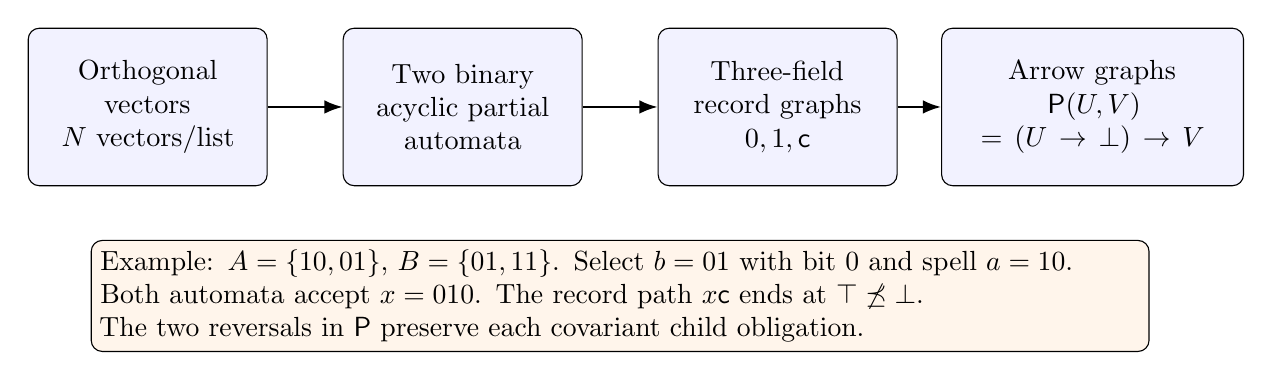
\begin{tikzpicture}[font=\normalsize,>=Latex,b/.style={draw,rounded corners,align=center,text width=28mm,minimum height=20mm,fill=blue!5},a/.style={->,thick}]
\node[b] (ov) at (0,0) {Orthogonal\\vectors\\$N$ vectors/list};
\node[b] (dfa) at (4,0) {Two binary\\acyclic partial\\automata};
\node[b] (rec) at (8,0) {Three-field\\record graphs\\$0,1,\checkfield$};
\node[b,text width=36mm] (arr) at (12,0) {Arrow graphs\\$\mathsf P(U,V)$\\$=(U\to\bot)\to V$};
\draw[a](ov)--(dfa);\draw[a](dfa)--(rec);\draw[a](rec)--(arr);
\node[draw,rounded corners,fill=orange!8,align=left,text width=132mm] at (6,-2.4) {Example: $A=\{10,01\}$, $B=\{01,11\}$. Select $b=01$ with bit $0$ and spell $a=10$.\\Both automata accept $x=010$. The record path $x\checkfield$ ends at $\top\not\Sub\bot$.\\The two reversals in $\mathsf P$ preserve each covariant child obligation.};
\end{tikzpicture}
\caption{Main reduction. The automata hardness is prior context~\cite{DDFMW25}; the record acceptance test and arrow embedding transfer it to the type semantics. The instance size is $\Oh(Nd+N+\log N)$ before the constant-overhead type encodings.}
\label{fig:reduction}
\end{figure}

The upper-bound pipeline tests equality, constructs equality quotients, and searches their directed product. If the quotient sizes are $q_G,q_H$, at most $2q_Gq_H\le 2nr$ normalized states are available. This parameter counts distinguishable regular-tree states, whereas feedback width counts cycles. The lower bound separates their roles: both feedback widths are zero on the hard family.

\begin{table}[H]
\caption{Quantitative context. $n$ counts type-graph vertices and edges; $M,B$ are the type-size and binder parameters used by QuickSub. The automata row is prior work, not a new hardness premise.}
\label{tab:map}
\centering
\begin{tabular}{p{.29\textwidth}p{.23\textwidth}p{.39\textwidth}}
\toprule
Problem / source & Bound & Representation / scope\\\midrule
Amadio--Cardelli~\cite{AC93} & Exponential & Equi-recursive arrow subtyping\\
KPS~\cite{KPS93,KPS95} & $\Oh(|G||H|)$ & Shared graphs; polarity product\\
Hopcroft--Karp method~\cite{HK71} & $\Oh(n\alpha(n))$ here & Unfolding equality\\
Palsberg--Zhao~\cite{PZ01} & Quadratic & Matching modulo additional product laws\\
QuickSub~\cite{QuickSub25} & $\Oh(MB)$ & Iso-recursive Amber relation\\
\cite[Lemma 6.4]{DDFMW25} & No strongly subquadratic 2-IE, OVH & Binary finite-word automata\\\midrule
Theorem~\ref{thm:A} & No $\Oh(n^{2-\varepsilon})$, OVH & Acyclic records; arrows alone\\
Theorem~\ref{thm:B} & $\Oh(n\log n+nr)$ & Minimized product; recursion count insufficient\\
Theorem~\ref{thm:access} & $\Oh(n\min\{n,\pi\})$ & Acyclic side; linear on a tree side\\
\bottomrule
\end{tabular}
\end{table}
\FloatBarrier

\section{Model and the Product Characterization}\label{sec:model}
The surface type language is
\[
 T::=\top\mid\bot\mid X\mid T\to T\mid\rec{\ell_i:T_i}_{i\in I}\mid\mu X.T.
\]
Records have distinct labels and immutable, covariant fields. Recursive types are contractive: cycles pass through a constructor. We permit shared definitions, equivalently finite systems of guarded type equations with a designated root. This is a representation choice: a system can be unfolded into nested $\mu$ syntax, but that translation need not preserve size. An acyclic system uses no recursion at all, yet may share many subexpressions. Inputs are constructor graphs with variable aliases already resolved. Leaves have kind $\top$ or $\bot$; arrow nodes have domain and codomain edges; record nodes have labeled field edges. Bounded arity means a fixed upper bound on outgoing edges. Our lower bounds use at most three. The validation implementation also permits distinct atomic leaf names, comparable only to the same name or through $\bot,\top$; this extension leaves the arguments unchanged.

\paragraph{Semantics.}
Let $\mathcal V$ be the disjoint union of both graphs' vertices. Define a monotone operator $F$ on relations over $\mathcal V^2$. A pair $(s,t)$ is in $F(R)$ if any of the following holds:
\begin{enumerate}
\item $s$ has kind $\bot$, or $t$ has kind $\top$;
\item both are arrows, $(t_{\rm dom},s_{\rm dom})\in R$, and $(s_{\rm cod},t_{\rm cod})\in R$;
\item both are records, $\mathrm{lab}(t)\subseteq\mathrm{lab}(s)$, and $(s_\ell,t_\ell)\in R$ for every $\ell\in\mathrm{lab}(t)$.
\end{enumerate}
Subtyping $\Sub$ is the greatest fixed point $\nu F$. Rule 1 also gives $\top\Sub\top$ and $\bot\Sub\bot$. Equality $\eqt$ is equality of unfolded labeled constructor trees, with exactly matching record label sets. It is a different fixed-point specification and does not identify arbitrary comparable nodes. These definitions include the standard width, depth, and function-variance rules.

\paragraph{Normalized obligations.}
A search state is $(u,v,p)$ with $u\in G$, $v\in H$, and $p\in\{+,-\}$. Its meaning is $u\Sub v$ for $p=+$ and $v\Sub u$ for $p=-$. For a locally compatible arrow pair, the domain successor flips polarity and the codomain successor retains it. For records, use the label set required by the current right-hand side and preserve polarity. A $\bot$ left side or $\top$ right side is successful with no successors. A state is \emph{bad} if none of the local clauses applies.

\begin{lemma}[Bad-pair reachability]\label{lem:product}
A root judgment fails if and only if a bad state is reachable by obligation edges. There are at most $2\size{V_G}\size{V_H}$ states, and exploration takes $\Oh(\size G\size H)$ time and space at bounded arity.
\end{lemma}
\begin{proof}
Let $Q$ be the reachable obligation states. If no state in $Q$ is bad, orient its pairs according to polarity. The resulting relation $R$ satisfies $R\subseteq F(R)$: each state is locally compatible and every required successor belongs to $Q$. Thus the root is in $\nu F$. Conversely, every pair in $\nu F$ is locally compatible and all its obligations remain in $\nu F$. Induction on a path from the root excludes a reachable bad state. The bound counts the two polarities for each cross-graph vertex pair. At fixed arity each state has constant many obligations and constant local comparison cost. A dense indexed visited table gives deterministic constant-time membership operations. Each visited state is expanded once. This proves both correctness and the stated bounds.
\end{proof}

Successful cycles are justified coinductively by the entire closed relation, not by an assumption that directed subtyping is an equivalence. A predecessor pointer for each newly reached state yields a finite counterexample path on failure. Its length is less than the product-state bound after removing repeated states.


\section{The Conditional Lower Bound}\label{sec:lower}
We transfer finite-word automata hardness to the structural subtype relation. The automata step is included as a direct specialization for a self-contained proof. Lists may contain duplicate vectors.

\subsection{OV to two acyclic partial automata}
Let $A,B\subseteq\bits^d$ be lists of length $N$, and put $L=\lceil\log_2 N\rceil$. Assign distinct $L$-bit selectors $\operatorname{sel}(j)$ to $b_j\in B$. Consider the following languages of words of length $L+d$:
\begin{align*}
\mathcal L_A&=\{za: z\in\bits^L,\ a\in A\},\\
\mathcal L_B&=\{\operatorname{sel}(j)x: x\in\bits^d,\ x\cdot b_j=0\}.
\end{align*}
A partial deterministic automaton $D_A$ first consumes $L$ arbitrary bits using a chain whose two transitions at each step have the same destination. It then follows a binary trie for the distinct vectors of $A$. Its accepting states are exactly the depth-$d$ trie leaves. The selector chain uses $L$ nodes and the trie at most $1+Nd$ nodes.

Automaton $D_B$ has a trie for the $N$ selectors. At selector $j$, attach a private length-$d$ chain. At coordinate $i$, permit symbol 0 always and symbol 1 exactly if $(b_j)_i=0$. Both permitted symbols lead to the next chain node. Only chain endpoints accept. Missing selector strings and forbidden bits have undefined transitions. The selector trie has fewer than $2^{L+1}$ nodes and all private chains together have $Nd$ nodes. Both graphs are layered and acyclic; no rejecting sink is introduced.

\begin{lemma}\label{lem:ovdfa}
The two automata have $\Oh(Nd+N+\log N)$ total size and can be built in that time. Their languages intersect if and only if the OV instance contains an orthogonal pair.
\end{lemma}
\begin{proof}
A common word has a valid selector $\operatorname{sel}(j)$ because it is accepted by $D_B$, and its final $d$ bits form some $a\in A$ because it is accepted by $D_A$. The coordinate chain accepts that suffix exactly when $a_i(b_j)_i=0$ for every $i$, equivalently $a\cdot b_j=0$. Conversely, an orthogonal pair supplies the common word $\operatorname{sel}(j)a$. The construction and node bounds above use tries and chains of constant outdegree, so the edge count and construction time satisfy the same bound.
\end{proof}

\paragraph{Relationship to the existing automata construction.}
Lemma 6.4 of~\cite{DDFMW25} already gives the automata hardness premise. Its vector selectors and coordinate-responsibility checks progress through finitely many layers; rejecting transitions can be omitted. Binary encoding replaces transitions by finite gadgets. Thus acyclic partial automata are available from that construction as well. Our selector--vector word above is a direct binary specialization used to make the type encoding transparent. The type-specific steps are the harmless termination of missing transitions, the acceptance-field test, and the arrow-only embedding below.

\subsection{A three-field record encoding}
For a state $q$ of $D_A$, create a left record node $S_q$. For a state $q$ of $D_B$, create a right record node $T_q$. All record nodes have \emph{exactly} the same fields $0,1,\checkfield$. For $a\in\bits$ let
\begin{align*}
(S_q)_a&=\begin{cases}S_{\delta_A(q,a)}&\delta_A(q,a)\text{ defined},\\\bot&\text{otherwise},\end{cases}\\
(T_q)_a&=\begin{cases}T_{\delta_B(q,a)}&\delta_B(q,a)\text{ defined},\\\top&\text{otherwise}.\end{cases}
\end{align*}
The acceptance fields are
\[
(S_q)_{\checkfield}=\begin{cases}\top&q\in F_A,\\\bot&q\notin F_A,\end{cases}\qquad
(T_q)_{\checkfield}=\begin{cases}\bot&q\in F_B,\\\top&q\notin F_B.\end{cases}
\]
An undefined transition is therefore harmless on either side. A comparison of acceptance fields fails precisely on $\top\Sub\bot$.

\begin{lemma}[Intersection is failure]\label{lem:encoding}
For any states $p,q$ of the two partial automata,
\[
 S_p\not\Sub T_q\quad\Longleftrightarrow\quad
 \mathcal L(D_A,p)\cap\mathcal L(D_B,q)\ne\varnothing.
\]
The construction preserves acyclicity and increases graph size by a constant factor.
\end{lemma}
\begin{proof}
Until a transition is undefined, following fields 0 and 1 follows the synchronized automata. At the first undefined transition, the comparison has $\bot$ on the left or $\top$ on the right and no bad state can occur below it. At any pair of record states, the $\checkfield$ obligation is bad exactly when both states accept. Hence a common accepted word $x$ gives a bad path $x\checkfield$. Conversely, every bad path must end in this form: the records have matching fields, and all paths that leave synchronized record states through 0 or 1 into an undefined transition succeed. Thus a bad path identifies a word accepted by both automata. Apply Lemma~\ref{lem:product}. All new nonterminal nodes are records pointing along the old transitions, or to leaves; no new cycle is created.
\end{proof}

\subsection{Removing records entirely}
Define the covariant pair constructor, as an abbreviation over arrows,
\[
 \mathsf P(U,V)=(U\to\bot)\to V.
\]
For all types in our structural semantics,
\begin{equation}\label{eq:pair}
 \mathsf P(U,V)\Sub\mathsf P(U',V')
 \quad\Longleftrightarrow\quad U\Sub U'\ \land\ V\Sub V'.
\end{equation}
Indeed the outer domain comparison is $(U'\to\bot)\Sub(U\to\bot)$, whose domain comparison is $U\Sub U'$. Both codomain obligations $\bot\Sub\bot$ succeed. The outer codomain comparison is $V\Sub V'$.
Replace each three-field record by
\[
 E(\rec{0:U,1:V,\checkfield:W})
 =\mathsf P(E(U),\mathsf P(E(V),E(W))),
\]
and preserve $\top,\bot$. Use shared references to $E$ of each original node, so each record costs four arrow nodes.

\begin{lemma}\label{lem:arrows}
On the record graphs of Lemma~\ref{lem:encoding}, $S\Sub T$ if and only if $E(S)\Sub E(T)$. The encoding has constant size overhead, arity two, and preserves acyclicity.
\end{lemma}
\begin{proof}
All compared nonterminal record nodes have the same three fields. Equation~\eqref{eq:pair} makes their encoded comparison equivalent to the conjunction of exactly their three child comparisons. Comparisons involving $\bot$ or $\top$ have the same success or failure before and after encoding. For acyclic inputs, induction on the sum of remaining heights proves the equivalence. Acyclicity follows because each wrapper leads only inward to its own finite encoding or onward to encoded original successors. There are four arrow nodes per original record and two shared constant leaves. (The same preservation also follows coinductively on cyclic fixed-field graphs, but the lower bound needs only the acyclic case.)
\end{proof}

\begin{proof}[Proof of the lower-bound part of Theorem~\ref{thm:A}]
Fix $0<\varepsilon<1$. A larger saving would imply one in this range. Choose $c$ from OVH for saving $\varepsilon/2$. At $d=\lceil c\log_2N\rceil$, Lemmas~\ref{lem:ovdfa}--\ref{lem:encoding} construct an instance of size $n=\Oh(N\log N)$ with $S\Sub T$ exactly when the OV answer is no. A deterministic decision algorithm for subtyping also decides its complement with the same running time. A time bound $\Oh(n^{2-\varepsilon})$ would therefore decide OV in
\[
 \Oh(N\log N+(N\log N)^{2-\varepsilon})
 =\Oh(N^{2-\varepsilon/2}),
\]
contradicting Definition~\ref{def:ovh}. Lemma~\ref{lem:arrows} gives the same contradiction without records. Both automata are layered with height $L+d=\Oh(\log N)$. Record encoding adds only a constant to path length, and the arrow encoding multiplies it by a constant. The reachable coordinate chains of $D_B$ ensure $n\ge N$, so the hard type graphs have height $\Oh(\log n)$. The label and arity restrictions follow from the encodings.
\end{proof}


\section{Equality, Quotients, and Parameters}\label{sec:upper}

\begin{figure}[H]
\centering
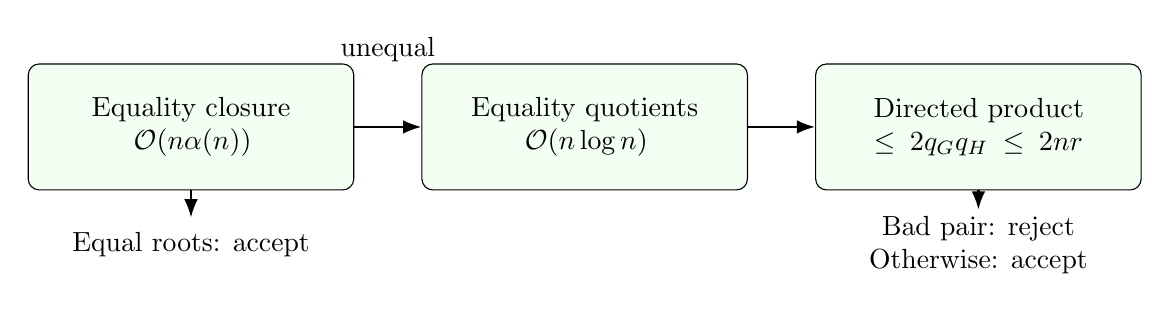
\begin{tikzpicture}[font=\normalsize,>=Latex,b/.style={draw,rounded corners,align=center,text width=39mm,minimum height=16mm,fill=green!5}]
\node[b](eq) at (0,0) {Equality closure\\$\Oh(n\alpha(n))$};
\node[b](min) at (5,0) {Equality quotients\\$\Oh(n\log n)$};
\node[b](prod) at (10,0) {Directed product\\$\le 2q_Gq_H\le 2nr$};
\draw[->,thick](eq)--node[above,yshift=7mm]{unequal}(min);
\draw[->,thick](min)--(prod);
\node[align=center] at (0,-1.5) {Equal roots: accept};
\draw[->,thick](eq)--(0,-1.15);
\node[align=center] at (10,-1.5) {Bad pair: reject\\Otherwise: accept};
\draw[->,thick](prod)--(10,-1.05);
\end{tikzpicture}
\caption{\musub\ uses classical equality and minimization before directed subtyping. Equality merges equivalence classes; the product retains directed obligations and a polarity bit.}
\label{fig:framework}
\end{figure}

\subsection{Why equality can use union-find}
An output signature comprises a node's constructor kind and exact set of outgoing edge names. Arrow edges are named domain and codomain. For equality, variance is irrelevant: corresponding subtrees must be equal in both positions.

\begin{algorithm}[H]
\caption{Unfolding equality (Hopcroft--Karp closure)}\label{alg:eq}
\begin{algorithmic}[1]
\State Initialize disjoint sets for all vertices; $W\gets[(s,t)]$
\While{$W$ is nonempty}
 \State Pop $(u,v)$ from $W$
 \State \textbf{if} $\operatorname{Find}(u)=\operatorname{Find}(v)$ \textbf{then continue}
 \State \textbf{if} output signatures differ \textbf{then return} \textsc{no}
 \State $\operatorname{Union}(u,v)$
 \State For each edge name $a$, push $(\delta(u,a),\delta(v,a))$ onto $W$
\EndWhile
\State \Return \textsc{yes}
\end{algorithmic}
\end{algorithm}

\begin{lemma}\label{lem:eq}
Algorithm~\ref{alg:eq} decides unfolding equality in $\Oh(n\alpha(n))$ time and $\Oh(n)$ space on bounded-arity graphs.
\end{lemma}
\begin{proof}
Suppose the roots are equal. Maintain that every generated obligation is an equal-tree pair and every union-find class contains equal trees. The invariant initially holds; equal nodes have the same output signature and equal corresponding successors. Union and successor generation preserve it, so the algorithm cannot reject.

Conversely, suppose it accepts. Let $M$ be the set of pairs whose processing performed a union, and let $C$ be the equivalence relation generated by $M$. Every pair in $M$ has equal output signatures. Any generated obligation is in $C$ at termination, since it either caused a union or was already in one class when popped. For every pair in $M$, corresponding successors are therefore in $C$. For an arbitrary pair in $C$, take a chain of pairs from $M$ and their reversals. Equal signatures propagate along the chain, and the corresponding successor chain witnesses $C$-related successors. Thus $C$ is a bisimulation of deterministic constructor graphs. Induction on finite tree depth shows that $C$-related nodes have identical truncations at every depth, hence identical unfoldings. The initial roots belong to $C$ at termination.

Every nontrivial iteration decreases the number of union-find classes. There are fewer than $n$ such iterations, each producing only constant many obligations at bounded arity. All other iterations consume those obligations. Weighted union with path compression gives $\Oh(n\alpha(n))$ total time; the sets, signatures, and worklist use linear space. This is the deterministic-automata equivalence closure underlying the Hopcroft--Karp method~\cite{HK71}.
\end{proof}
This proves the equality portion of Theorem~\ref{thm:A}. The proof uses transitive and symmetric closure of equality. A directed subtype assumption does not have those properties.

\subsection{Minimization and the regular-state upper bound}
The upper bound uses standard deterministic labeled-graph partition refinement~\cite{PT87}; the following proof records its correctness and scheduling invariant.

\begin{lemma}[Equality quotient]\label{lem:min}
For a bounded-arity constructor graph, the partition into equal unfolding trees is computable in time $\Oh(n\log n)$ and space $\Oh(n)$.
\end{lemma}
\begin{proof}
Initially partition nodes by output signature. Refine a partition whenever some nodes in a block have an edge of name $a$ into a block $B$ and others do not. Use inverse edge lists to compute $\operatorname{pre}_a(B)$, and split every block it intersects. A stable partition relates only equal unfoldings: related nodes have equal signatures and, for each edge name, successors in the same block. This is a bisimulation, so induction on depth establishes equality. Equal unfoldings can never be separated, initially or by a refinement, so stability gives precisely the desired partition.

Here is the standard smaller-half scheduling that provides the time bound. Initially enqueue every block as a splitter. Processing a splitter considers its incoming edges grouped by name. If a block awaiting processing is split, replace its queue entry by both children. If a block already processed is split, enqueue just its smaller child. Splitting a queued block only partitions its as-yet-unprocessed membership. After a vertex has belonged to a processed splitter, any new scheduled membership containing it has at most half the size of its previous such block. Thus each vertex and each incoming edge are charged $\Oh(\log n)$ times. Splits are maintained with block lists and per-vertex positions; a split costs time linear in the marked predecessors and in the number of new nonempty blocks. Sparse buckets for touched edge names avoid iterating over unused labels. Initial signatures can be sorted in $\Oh(n\log n)$ time; outgoing lists have constant length. Total edge and vertex charges give $\Oh(n\log n)$ time and linear working space.

It remains to justify the omission of the larger child. Partitions only refine. Once predecessor blocks are stable for a previously processed parent splitter, stability for one child implies stability for the other, since its predecessor set is the parent's predecessor set minus the child's, separately for each edge name. If the parent was still queued, both children are queued instead, so no required distinction is lost. Consequently an empty queue means the partition is stable, establishing the claimed algorithm and its bound.
\end{proof}

\begin{lemma}[Quotient substitution]\label{lem:quot}
Replacing either input by its unfolding-equality quotient preserves every root subtyping judgment.
\end{lemma}
\begin{proof}
The quotient map preserves each constructor, label set, and successor class. Lift a post-fixed subtype relation on quotient nodes to all pairs of their original nodes; the clauses of $F$ hold because outputs and successor classes are preserved. This proves one implication by the greatest-fixed-point property. For the other implication, map all pairs of an original post-fixed relation to their quotient classes. Any witness pair for a class pair has the same local constructors and the same successor classes as every other representative, so its required successors appear in the image relation. This image is post-fixed. Applying these two constructions to $\nu F$ proves both directions.
\end{proof}

\begin{proof}[Proof of the upper bound in Theorem~\ref{thm:B}]
First test equality by Lemma~\ref{lem:eq}, if desired. If unequal, minimize both reachable graphs using Lemma~\ref{lem:min} and run the obligation search of Lemma~\ref{lem:product}. By Lemma~\ref{lem:quot} its answer is unchanged. Write $q_G=r(G)$ and $q_H=r(H)$. Bounded arity gives quotient sizes $\Oh(q_G)$ and $\Oh(q_H)$. Since $\max(q_G,q_H)\le n$,
\[
 2q_Gq_H\le 2nr.
\]
The running time is $\Oh(n\log n+nr)$ and space is $\Oh(n+nr)$. The optional equality test fits within these bounds.
\end{proof}

\paragraph{Exponent optimality has a specific meaning.}
Suppose that a uniform algorithm had time $\Oh((nr)^{1-\varepsilon})$ on all instances. Since $r\le n$, it would take $\Oh(n^{2-2\varepsilon})$ on the lower-bound family, contradicting Theorem~\ref{thm:A}. Likewise, $\Oh(n\log n+n r^{1-\varepsilon})$ is at most $\Oh(n\log n+n^{2-\varepsilon})$. An algorithm may read the input in $\Oh(n)$ time in either case; this does not change the contradiction for $0<\varepsilon<1/2$. Larger savings imply one in this range. These are global exponent barriers, rather than tight lower bounds for all parameter slices.

\subsection{Why counting recursion alone fails}
\begin{proof}
Every graph in Lemma~\ref{lem:encoding} is acyclic, hence has feedback width zero on both sides. The proposed feedback-parameter bound specializes to near-linear time on this family, contradicting Theorem~\ref{thm:A}. Every node can also be named by an acyclic, nonrecursive type definition in topological order. Such an input has zero $\mu$-binders when sharing definitions are allowed. Thus counting recursive binders has the same defect. The arrow-only encoding preserves acyclicity, so record width subtyping is not responsible for this obstruction.
\end{proof}

This conditional impossibility concerns a running-time guarantee. One can also refute the proposed bound on \emph{reachable product states} unconditionally. Consider coprime positive integers $p,q$ and the unary recursive records
\[
 A_i=\rec{a:A_{i+1\bmod p}},\qquad
 B_j=\rec{a:B_{j+1\bmod q}}.
\]
From $(A_0,B_0)$ the orbit has $\operatorname{lcm}(p,q)=pq$ distinct pairs. Each input cycle has a single feedback edge. Yet all nodes unfold to the same unary infinite tree, so equality closure accepts in near-linear time and both quotients have one state. This example distinguishes an algorithm-specific product-size obstruction from a decision lower bound.

\subsection{A finite-access guarantee}
\begin{proof}[Proof of Theorem~\ref{thm:access}]
Unfold the acyclic side $K$ into a finite tree $\widehat K$ by making one copy of a node for each root-to-node path. Its number of nodes is
\[
 U(K)=\sum_{v\in V_K}\#\{\text{root-to-}v\text{ paths}\}
 \le\size{V_K}\pi(K).
\]
At bounded arity its edge count is of the same order. Each tree occurrence has a unique path from the root. The obligation transition on the other graph is deterministic for each edge name, and domain edges determine the polarity flip. Therefore every occurrence can be compared to at most one other-graph node with one polarity. Local success may stop a path early, and a missing required field may reject earlier; neither increases the count. Enumerating occurrences on demand costs $\Oh(U(K))$, after input reading. If a required record edge is missing on the tree side, reject at that occurrence rather than unfolding anything further.

Alternatively use the ordinary product algorithm for $\Oh(n^2)$ time. Choose between the two using $\pi(K)$ capped at $n$. In a topological ordering, initialize the root path count to one and all others to zero; send each count along every outgoing edge, saturating every addition at $n$. Induction on the order shows the resulting values equal the true counts capped at $n$. This requires constant-word arithmetic per edge and computes the capped maximum in $\Oh(n)$ time. Choosing the smaller of the two bounds gives $\Oh(n\min\{n,\pi(K)\})$. For a rooted tree every reachable node has one root path, so the result is linear.
\end{proof}




\begin{table}[H]
\centering
\begin{tabular}{ll}
\toprule
Structural graph model & Complexity guarantee\\\midrule
Unfolding equality & $\Oh(n\alpha(n))$\\
Unrestricted subtyping & $\Oh(n^2)$; OVH barrier\\
Smaller quotient size $r$ & $\Oh(n\log n+nr)$\\
One explicit tree side & $\Oh(n)$\\\bottomrule
\end{tabular}
\caption{Complexity within the main semantic model. The Boolean-record set interpretation is developed separately in Appendix~\ref{sec:boolean}.}
\label{tab:complexity}
\end{table}

\FloatBarrier

\section{Executable Validation}\label{sec:exp}
The artifact implements the shared-graph semantics, the OV encodings, equality closure, and two equality-quotient routines. We use sparse smaller-half partition refinement for the revised \musub\ pipeline and retain Moore refinement as a differential oracle. The splitter snapshots incoming edges before refining its current block and schedules smaller children as in Lemma~\ref{lem:min}. Its counters record incoming-edge visits, splitter memberships, and moved vertices. JavaScript Map/Set operations are supplied by the runtime; the RAM analysis in the theorem concerns the abstract partition data structures.

\paragraph{Correctness checks.}
All $225$ pairs of nonempty subsets of $\bits^2$ agree between direct OV enumeration, record subtyping, and quotient subtyping. The arrow encoding passes the same $225$ cases. A descending fixed-point oracle independently decomposes the type rules and agrees with product and quotient decisions on $2,000$ seeded cyclic queries. Equality is also checked by synchronized exploration. A further $3,000$ seeded random graphs give the same quotient sizes under smaller-half and Moore refinement, and all returned blocks satisfy successor stability. The seeds are $1701$ and $20271031$, respectively. Cycles of lengths $17$ and $19$ yield exactly $323$ baseline product states.

\paragraph{Synthetic family and measurement protocol.}
For $N=2^L$, use
\[
 a_i=(\operatorname{bin}_L(i),0^L,1),\qquad
 b_j=(0^L,\operatorname{bin}_L(j),1).
\]
Every pair overlaps in its final coordinate, so subtyping succeeds after the reduction. The family deliberately exposes repeated selector/vector comparisons, while identical suffixes make equality quotienting effective. The baseline is our KPS-style graph product implementation. Runs use Node.js v25.5.0 on an Apple M3 Pro (arm64), with two warmups and seven measured repetitions at each size. Input generation is excluded. \musub\ timings include equality, both quotient constructions, and the quotient-product search. Raw per-run observations are retained.

\begin{table}[H]
\centering
\begin{tabular}{rrrrrrrr}\toprule
$N$ & $n_v$ & $n_e$ & $n$ & $r$ & $P_{\rm base}$ & $P_{\rm quot}$ & $2q_Gq_H$\\\midrule
16 & 294 & 870 & 1,164 & 16 & 1,600 & 128 & 3,616\\
32 & 679 & 2,025 & 2,704 & 19 & 7,312 & 288 & 9,766\\
64 & 1,544 & 4,620 & 6,164 & 22 & 33,088 & 640 & 25,388\\
128 & 3,465 & 10,383 & 13,848 & 25 & 148,160 & 1,408 & 64,050\\
256 & 7,690 & 23,058 & 30,748 & 28 & 656,896 & 3,072 & 157,752\\
\bottomrule\end{tabular}
\caption{Input size and actual expanded normalized states on the synthetic family. The theoretical size is $n=n_v+n_e$ in every row. $P_{\rm base}$ uses the original graphs; $P_{\rm quot}$ uses the quotients. The last column is the exact quotient state-space bound.}
\label{tab:states}
\end{table}
\begin{table}[H]
\centering
\begin{tabular}{rrrrrr}\toprule
$N$ & Baseline & Equality & Minimization & Search & Total \musub\\\midrule
16 & 0.775 & 0.077 & 0.474 & 0.066 & 0.620\\
32 & 2.613 & 0.175 & 1.071 & 0.096 & 1.409\\
64 & 14.077 & 0.582 & 2.957 & 0.215 & 3.776\\
128 & 91.999 & 0.961 & 5.340 & 0.639 & 6.818\\
256 & 460.842 & 2.167 & 14.982 & 1.584 & 18.736\\
\bottomrule\end{tabular}
\caption{Measured phase times in milliseconds, with seven-run medians. Total times the full \musub\ pipeline; separate phase medians need not add to it. These measurements use smaller-half refinement.}
\label{tab:phases}
\end{table}


Table~\ref{tab:states} separates the baseline search from the search constrained by the theorem. For example, at $N=256$, the baseline expands $656,896$ states, whereas the quotient search expands $3,072$. The latter is below the exact state-space limit $2q_Gq_H=157,752$. The theorem bounds this quotient search; the baseline uses the original graphs. Table~\ref{tab:phases} exposes the cost paid to obtain that reduction. All reported phases are measured directly with the revised splitter implementation.

\begin{figure}[H]
\centering
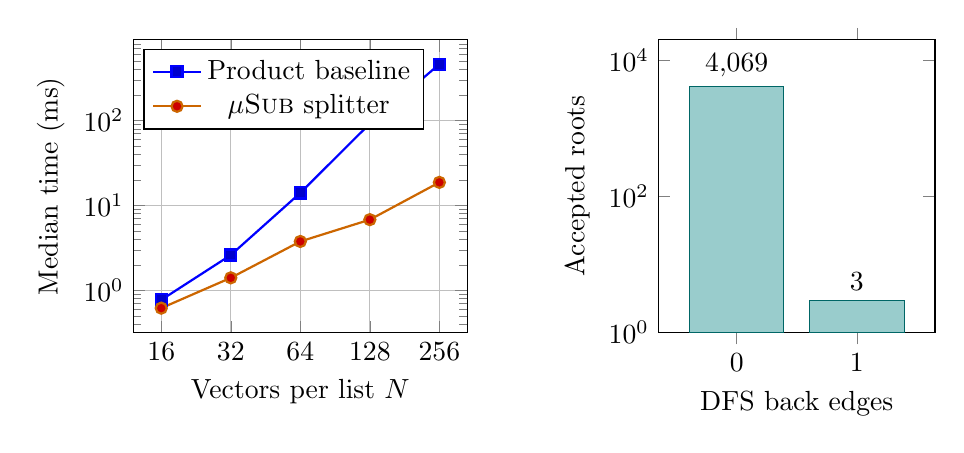
\begin{tikzpicture}
\begin{axis}[width=.48\textwidth,height=53mm,xmode=log,log basis x=2,ymode=log,
 xlabel={Vectors per list $N$},ylabel={Median time (ms)},xtick={16,32,64,128,256},
 xticklabels={16,32,64,128,256},legend pos=north west,legend style={font=\normalsize},
 grid=major,tick label style={font=\normalsize},label style={font=\normalsize}]
\addplot+[mark=square*,blue,thick] coordinates {(16,0.775042) (32,2.613208) (64,14.077417) (128,91.998584) (256,460.842)};
\addlegendentry{Product baseline}
\addplot+[mark=*,orange!80!black,thick] coordinates {(16,0.619833) (32,1.4095) (64,3.776375) (128,6.817959) (256,18.735667)};
\addlegendentry{\musub\ splitter}
\end{axis}
\begin{axis}[at={(.55\textwidth,0)},anchor=south west,width=.42\textwidth,height=53mm,
 ybar,bar width=12mm,ymode=log,ymin=1,ymax=20000,xmin=-.65,xmax=1.65,
 xtick={0,1},xticklabels={0,1},xlabel={DFS back edges},
 ylabel={Accepted roots},ytick={1,100,10000},
 tick label style={font=\normalsize},label style={font=\normalsize},log origin=infty]
\addplot[fill=teal!40,draw=teal!80!black] coordinates {(0,4069)(1,3)};
\node[above,font=\normalsize] at (axis cs:0,4069) {4,069};
\node[above,font=\normalsize] at (axis cs:1,3) {3};
\end{axis}
\end{tikzpicture}
\caption{Left: newly measured times on the compressible synthetic family, including all \musub\ phases. Right: DFS counts only for the $4,072$ extracted corpus roots, or $6.79\%$ of candidates. Both vertical axes are logarithmic.}
\label{fig:experiments}
\end{figure}


\paragraph{Corpus scan and coverage.}
A pinned DefinitelyTyped snapshot~\cite{DT} supplies $23,098$ declaration files. Of $59,949$ file-top-level interface/alias candidates, $4,072$ pass the closed monomorphic projection ($6.79\%$). Among accepted roots, $4,069$ have no DFS back edges and three have one. Equality-quotient sizes are 1--4 for $4,007$ roots, 5--16 for $64$, and 17--64 for one. Figure~\ref{fig:experiments} shows the measured subset; Appendix~\ref{sec:artifact} gives its exact extraction boundary, commit, digest, and commands.

\paragraph{Interpretation and limitations.}
The synthetic results explain a mechanism---fewer distinct comparison states after quotienting---on a compressible family. The corpus counts describe the accepted projection: generics, optional members, and other excluded constructs introduce substantial selection bias. Neither experiment estimates end-to-end compiler performance or supplies evidence for OVH. Smaller-half refinement aligns the implementation with the analyzed scheduling rule; finite timing data remain separate from the asymptotic proof. These are standalone graph-checker measurements, with TypeScript and Scala-like parsers used only as explicit projections.
\FloatBarrier

\section{Consequences and Further Questions}\label{sec:related}
The conditional quadratic barrier for shared acyclic types survives both a fixed record signature and elimination of records. Sharing can therefore create the hard interaction even when feedback width is zero. The companion tree-side upper bound shows why this conclusion depends on representation. A unary pair of cycles illustrates a different phenomenon: a raw product may be quadratic while equality collapses both inputs immediately.

The result is a type-semantic transfer of the established automata premise, rather than an improvement of the automata lower bound. Palsberg and Zhao's flexible matching~\cite{PZ01} and QuickSub's iso-recursive Amber relation~\cite{QuickSub25} address different equivalences or subtyping rules. For the present relation, equality quotienting offers a standard state-sensitive guarantee, while finite access provides a more syntactic guarantee for acyclic inputs.

Three questions remain. Can a useful binder-sensitive bound be proved for explicit nested $\mu$ syntax when nonrecursive sharing is forbidden? Can a parameter smaller than the minimal regular-tree state count handle large but simple periodic structures? Which support parameter works for fully specified recursive set-theoretic function types? The finite Boolean-record result in Appendix~\ref{sec:boolean} isolates a modest specialization of the last question.

\clearpage
\appendix
\section{Boolean-Record Support Width: A Separate Extension}\label{sec:boolean}
This appendix studies a finite set interpretation of records. It is independent of the coinductive structural relation used in the main text. Boolean support, rather than union-node fan-in, controls its exhaustive decision procedure.
For unions, we explicitly restrict the semantics. A Boolean record is a fixed binary tree with $w$ free Boolean leaves. An atom $P_i^e$ tests whether leaf $i$ contains the singleton bit $e$. Types are formulas of these atoms using binary union and intersection, interpreted as sets of Boolean records. The \emph{support width} is the number of leaf coordinates mentioned, not the arity of a union constructor. Let $m$ count the formula DAGs and their atom descriptions.

\begin{theorem}[Boolean support width]\label{thm:C}
In this Boolean-record fragment, semantic subtyping is decidable in $\Oh(2^w m)$ time. Under ETH it has no $2^{o(w)}m^{\Oh(1)}$ algorithm. If union width means only the maximum union-node arity, subtyping is coNP-complete even when that width is two. The hardness uses only two record labels and arity two.
\end{theorem}
The universe and operations below specify the entire semantic fragment; general set-theoretic function types require further realizability machinery~\cite{FCB08}.



\paragraph{Boolean-record universe.}
Let $h=\lceil\log_2\max\{2,w\}\rceil$ and let $\mathcal U_w$ contain full binary record trees of depth $h$, with Boolean singleton leaves $\mathbf 0,\mathbf 1$. The first $w$ leaves vary independently and any remaining leaves are fixed to $\mathbf0$. Record labels at internal nodes are just 0 and 1. The universe has exactly $2^w$ values. It can be described by a shared record schema of $\Oh(w)$ size. The singleton bit types are additional constants of this separate fragment, with their literal set interpretation.

The atom $P_i^e$ is the subset of $\mathcal U_w$ whose $i$th leaf is $\mathbf e$. It can be written as the nested open-record constraint following the $h$-bit address of $i$, ending in $\mathbf e$; all other branches are unspecified. This uses $\Oh(\log(w+1))$ nodes and the two fixed labels. Formulas use $P_i^0,P_i^1$, the empty and universal sets relative to $\mathcal U_w$, and binary $\cup,\cap$. Their denotations are given by ordinary set union and intersection. Subtyping $S\le_{\mathcal U_w}T$ means inclusion of these denotations. If formulas mention fewer than $w$ distinct coordinates, discard the unused coordinates; this gives the support-width parameter in Theorem~\ref{thm:C}.

\begin{proof}[Proof of Theorem~\ref{thm:C}]
For the upper bound, enumerate the $2^w$ assignments to the mentioned coordinates. Evaluate every atom, then every union/intersection node in topological order. Reject inclusion if $S$ evaluates to true and $T$ to false for some assignment; otherwise accept. Evaluation costs $\Oh(m)$ per assignment even if atoms are stored as explicit paths, and uses $\Oh(m+w)$ working space.

For the lower bound, take a 3-CNF formula $\varphi$ on $w$ Boolean variables. Translate a positive literal $x_i$ to $P_i^1$, a negative literal $\neg x_i$ to $P_i^0$, a disjunction to a binary-union tree, and a conjunction to a binary-intersection tree. Call the result $T_\varphi$. For each assignment $a$, the corresponding record belongs to $T_\varphi$ exactly when $\varphi(a)$ is true, by structural induction on the formula. Consequently
\[
 T_\varphi\le_{\mathcal U_w}\varnothing
 \quad\Longleftrightarrow\quad\varphi\text{ is unsatisfiable}.
\]
The type description has size polynomial in the CNF input and $w$; shared literal definitions can be reused. A $2^{o(w)}m^{\Oh(1)}$ subtyping algorithm, followed by complementing its answer, would decide 3-SAT in subexponential variable time, contradicting ETH~\cite{IP01}. All unions are binary and internal records have arity two with just labels 0 and 1.

Finally, a failure of inclusion has a polynomial-size certificate: an assignment to the mentioned coordinates. Its evaluation takes polynomial time. Thus inclusion is in coNP. The same reduction from 3-UNSAT proves coNP-hardness when the maximum union arity is two. This establishes the last claim as well as the exponential support-width barrier.
\end{proof}



\section{Artifact, Data Provenance, and Projection Boundary}\label{sec:artifact}
\paragraph{Release.}
The accompanying artifact is available at \url{https://github.com/ArtificialZeng/musub-artifact/tree/musub-r2}, release \texttt{musub-r2}. The release points to commit \path{87ad1b7f6e5c603a94bdbe2e1fb6a71cc70c8f2c} and supplies a SHA-256 manifest covering source, raw timings, and corpus summaries. The same files are included in the accompanying source bundle. Its README distinguishes the measured splitter pipeline from the retained Moore reference.

\paragraph{Reproduction.}
From the repository root, the principal commands are:
\begin{quote}\ttfamily
npm ci\\
node validate.mjs\\
node validate-splitter.mjs\\
node extra-validation.mjs\\
node frontend-validation.mjs\\
node bench.mjs
\end{quote}
The first two validation seeds are recorded in \texttt{validation.json} and \texttt{splitter-validation.json}. \texttt{bench-results.json} contains each measured repetition and the summary medians, including $n_v,n_e,n,r$, both visited-state counts, exact quotient-product bounds, and phase timings. The phase medians need not sum to the median total; the total is timed independently over the whole pipeline.

\paragraph{Corpus identity.}
The DefinitelyTyped commit is
\begin{quote}\ttfamily\path{72e15dbdd8088284d3f0387a05539e7c2e6c743b}.\end{quote}
The ordered relative-path/content digest of the scanned files is
\begin{quote}\ttfamily\path{a2e28632e9fd2a9d838ac94f0c7afaee8bbd3acd2249cb77978390a85e0b4ce4}.\end{quote}
The README gives a pinned download command. Running \texttt{corpus.mjs} on the snapshot's \texttt{types/} directory recreates \texttt{corpus-summary.json}, \texttt{corpus-roots.json}, and \texttt{corpus-queries.json}. The first records coverage and bins, the second every accepted root, and the third the artificial adjacent-root queries.

\paragraph{TypeScript projection.}
The extractor uses TypeScript 5.9.3's syntax API. It accepts required record properties, primitive leaf names, unary functions, unknown/never, and file-local nongeneric references. It rejects inheritance, merged declarations, imports, nested declarations, generics, optional members, unions, and unsupported dependencies. Fields are projected to immutable fields and primitive names to distinct atoms; this also changes some tsc assignability rules for empty records and void. The scan measures a graph-model projection, with coverage reported against its file-top-level candidate set.

Per-root DFS finds one back edge in each accepted cyclic root from kuromoji, microsoftteams, and requirejs. DFS back-edge counts are a traversal statistic; zero certifies acyclicity, while general minimum feedback width is a different graph parameter. The accepted roots have the following histograms:
\begin{center}
\begin{tabular}{llr}\toprule
Statistic & Bin & Roots\\\midrule
DFS back edges & 0 & 4,069\\
 & 1 & 3\\\midrule
Equality-quotient states & 1--4 & 4,007\\
 & 5--16 & 64\\
 & 17--64 & 1\\
 & $\ge65$ & 0\\\bottomrule
\end{tabular}
\end{center}
Artificial comparisons between adjacent accepted roots in each file generated $2,510$ queries. The retained single-pass baseline latencies have $p_{50}=0.458\,\mu$s, $p_{90}=3.416\,\mu$s, and $p_{99}=19.542\,\mu$s. They are sensitive to timer and JIT overhead and do not represent compiler query traces.

\paragraph{Scala-like equations and frontend checks.}
The second parser accepts explicit type equations with val record fields, unary arrows, Any, and Nothing, as an interchange notation for the graph model. It does not implement Scala's path-dependent or full recursive-type semantics. Recursive payload examples yield four expected directional judgments across the two parsers. TypeScript 5.9.3 also checks \texttt{example.ts} under strict settings, including the expected failure of the reverse assignment. No compiler timing is inferred from these correctness checks.

\section*{AI Methodology}
OpenAI Codex materially assisted with the mathematical constructions, proof drafting, reference searches, implementation, experiments, and LaTeX revision. Verification records identify the mathematical arguments, independently coded fixed-point checks, differential quotient checks, source comparisons, and measured data used in this preparation. These records provide an auditable workflow; independent human proof and originality review is a separate author responsibility.

\clearpage
\bibliographystyle{alphaurl}
\bibliography{references}
\end{document}
